\documentclass[12pt]{article}
\usepackage{graphicx} % Required for inserting images
\usepackage{tikz}
\usetikzlibrary{external}
\tikzexternalize[prefix=tikz/]
\usepackage[utf8]{inputenc}
\usepackage{placeins}
\usepackage{longtable}
\usepackage{setspace}
\usepackage{multirow}
\usepackage{array}
\usepackage{blindtext}
\usepackage{listings}
\usepackage[backend = biber, style= mla]{biblatex}
\bibliography{refs}
\usepackage{csquotes}
\usepackage{amsmath}
\usepackage{amssymb}
\usepackage{pgfplots}
\setstretch{1.157}
 \usepackage{amsfonts}
\usepackage{tikz}
\usepackage{hyperref}
    \hypersetup{
    colorlinks=true,
    breaklinks=true,
    citecolor=blue,
    linkcolor=black,
    urlcolor=blue,
    }
\numberwithin{equation}{section}
\usepackage[nottoc, notlot, notlof, numbib]{tocbibind}
\usepackage[labelfont=bf]{caption}
\NeedsTeXFormat{LaTeX2e}
\ProvidesPackage{main}[2023/05/23 baskerville's Package]
%%Package options
%% This loads all the requiered packages for a proper compilation. However
%% future versions may affect the processing of the document. Therefore, it
%% TODO add version dates to all packages
%% TODO add warnings for outdated packages
\usepackage{etoolbox} %% Control sequence commands
\usepackage{lipsum} %% Lorem ipsum generator
\usepackage{ragged2e} %% For justifying text in Math IA's
\usepackage{lastpage} %% For retriving the total number of pages in the
%% typeset document
\usepackage[siunitx]{circuitikz} %[symbols]
\usepackage[outline]{contour} % glow around text
\usetikzlibrary{arrows,arrows.meta}
\usetikzlibrary{decorations.markings}
\tikzset{>=latex} % for LaTeX arrow head
\usepackage{xcolor}
\colorlet{Icol}{blue!50!black}
\colorlet{Ccol}{orange!90!black}
\colorlet{Rcol}{green!50!black}
\colorlet{loopcol}{red!90!black!25}
\colorlet{pluscol}{red!60!black}
\colorlet{minuscol}{blue!60!black}
\newcommand\EMF{\mathcal{E}} %\varepsilon}
\contourlength{1.5pt}
\tikzstyle{EMF}=[battery1,l=$\EMF$, invert]
\tikzstyle{internal R}=[R,color=Rcol,Rcol,l=$r$,/tikz/circuitikz/bipoles/length=30pt]
\tikzstyle{loop}=[->,red!90!black!25]
\tikzstyle{loop label}=[loopcol,fill=white,scale=0.8,inner sep=1]
\tikzstyle{thick R}=[R,color=Rcol,thick,Rcol,l=$R$]
\tikzstyle{thick C}=[C,thick,color=Ccol,Ccol,l=$C$]
\tikzstyle{myswitch}=[closing switch,line width=0.3] %-{Latex[length=3]},
\DeclareMathOperator\arctanh{arctanh}
\newcommand{\myvoltmeter}[2] 
{  % #1 = name , #2 = rotation angle
  \begin{scope}[transform shape,rotate=#2]
  \draw[thick] (#1)node(){$\mathbf V$} circle (11pt);
  \draw[rotate=45,-latex] (#1)  +(-17pt,0) --+(17pt,0);
  \end{scope}
}
\ctikzset{bipoles/thickness=1.2}
\newcommand{\midlabelline}[3]{
   \node (midlabel) at ($ (#1)!.5!(#2) $) {#3};
   \draw[latex-] (#1) --  (midlabel);
   \draw[-latex] (midlabel) -- (#2);
}
\makeatletter
\renewcommand{\@floatboxreset} {%
        \reset@font
        \normalsize
        \@setminipage
\centering%<<<<<<<<<<<<<<<<<<<
}
\makeatletter
\usepackage{graphicx} % Required for inserting images
\usepackage{tikz}
\usetikzlibrary{external}
\tikzexternalize[prefix=tikz/]
\usepackage[utf8]{inputenc}
\usepackage{placeins}
\usepackage{longtable}
\usepackage{setspace}
\usepackage[backend = biber]{biblatex}
\usepackage{csquotes}
\usepackage{multicol}
\usepackage{mhchem}
\addbibresource{refs.bib}
\RequirePackage{newfloat} %% For placing figures in the right place
\usepackage{fancyhdr} %% For custom headers and footers
\usepackage{caption} %% For custom captions
\usepackage[top=1in,bottom=1in,left=0.75in,right=0.75in]{geometry} 
\usepackage{array}
\usepackage[T1]{fontenc}
\usepackage[english]{babel}
\usepackage{graphicx}
\usepackage{soul}
\sethlcolor{green}
\usepackage{appendix}
\usepackage{subcaption}
\usepackage{multirow}
\usepackage{float}
\usepackage{physics}
\usepackage{makecell}
\usepackage[makeroom]{cancel}
\usepackage{enumerate}
\usepackage{hyperref}
    \hypersetup{
    colorlinks=true,
    breaklinks=true,
    citecolor=blue,
    linkcolor=black,
    urlcolor=blue,
    }
\numberwithin{equation}{section}
\usepackage[nottoc, notlot, notlof, numbib]{tocbibind}
\usepackage[labelfont=bf]{caption}
\usepackage{amsfonts,amsmath,amssymb}
\usepackage{fancyhdr} %Fancy Title 
\usepackage{setspace}
\usepackage{array}
    \newcolumntype{P}[1]{>{\centering\arraybackslash}p{#1}}
    \newcolumntype{M}[1]{>{\centering\arraybackslash}m{#1}}
\usepackage{multirow}
\usepackage{blindtext}
\usepackage{listings}
\usepackage{pgfplots}
\usepackage[siunitx]{circuitikz} %[symbols]
\usepackage[outline]{contour} % glow around text
\usetikzlibrary{arrows,arrows.meta}
\usetikzlibrary{decorations.markings}
\tikzset{>=latex} % for LaTeX arrow head
\usepackage{xcolor}
\colorlet{Icol}{blue!50!black}
\colorlet{Ccol}{orange!90!black}
\colorlet{Rcol}{green!50!black}
\colorlet{loopcol}{red!90!black!25}
\colorlet{pluscol}{red!60!black}
\colorlet{minuscol}{blue!60!black}
\contourlength{1.5pt}
\tikzstyle{EMF}=[battery1,l=$\EMF$, invert]
\tikzstyle{internal R}=[R,color=Rcol,Rcol,l=$r$,/tikz/circuitikz/bipoles/length=30pt]
\tikzstyle{loop}=[->,red!90!black!25]
\tikzstyle{loop label}=[loopcol,fill=white,scale=0.8,inner sep=1]
\tikzstyle{thick R}=[R,color=Rcol,thick,Rcol,l=$R$]
\tikzstyle{thick C}=[C,thick,color=Ccol,Ccol,l=$C$]
\tikzstyle{myswitch}=[closing switch,line width=0.3] %-{Latex[length=3]},

\renewrobustcmd{\footcite}[1]{
    \footcite{#1}
}


\floatplacement{graph}{H} %% Graphs are placed in the right place


\makeatletter
\renewcommand{\@floatboxreset} {%
        \reset@font
        \normalsize
        \@setminipage
\centering%<<<<<<<<<<<<<<<<<<<
}
\makeatletter

\DeclareFloatingEnvironment{graph}




%% Table of contents options
\renewrobustcmd{\tableofcontents}{
    \pagestyle{empty}
    \section*{Table of Contents}
    \vspace*{0.5cm}
    \hrule
    \vspace*{0.5cm}
    \@starttoc{toc}
    \newpage
    \setcounter{page}{1}
    \pagestyle{fancy}
    \restoregeometry
}

\NeedsTeXFormat{LaTeX2e}
\ProvidesPackage{main}[2023/05/23 baskerville's Package]
%%Package options
%% This loads all the requiered packages for a proper compilation. However
%% future versions may affect the processing of the document. Therefore, it
%% TODO add version dates to all packages
%% TODO add warnings for outdated packages
\RequirePackage{etoolbox} %% Control sequence commands
\RequirePackage{lipsum} %% Lorem ipsum generator
\RequirePackage{ragged2e} %% For justifying text in Math IA's
\RequirePackage{lastpage} %% For retriving the total number of pages in the
%% typsset document
\babelprovide[import,main]{english} %% Main language
\justifying %% This is a must for Math IA's, and is loaded from the ragged2e:
%% https://ctan.org/pkg/ragged2e?lang=en.

\fancyhead[C]{\small\scshape\@title} %% The title of the document is placed
%% in the center of the header. This is completly optional, and can be removed.
\fancyhead[R]{\small\scshape{\thepage/\pageref{LastPage}}} %% The page number
%% along with the total number of pages is placed in the right side of the
%% footer. This isnt required, but is an asthetic choice.
\fancyfoot{\hrule}


\newcommand{\uvec}[1]{\boldsymbol{\hat{\textbf{#1}}}}

\usepackage{hyperref}
\usepackage{pgfplots}
\pgfplotsset{compat=newest}
\usepackage{chemfig}
\usepackage{tcolorbox}
\title{Which Type of Magnetic Nanoparticle Is Most Effective For Induced-Hyperthermia Cancer Treatment?}
\date{\LARGE{}}
\begin{document}
\maketitle
\section{Introduction}
Despite the universal prevalence of cancer as a cause of mortality, there exist little to no treatments that can truly aid the afflicted with no significant, negative ramifications. Consider radiation and chemotherapy, generally the most popular forms of conventional treatment. Both of their detrimental effects manifest in the patient's bone marrow. Neutrophils are the initiators of the innate immune system, a type of “white blood cells” that are constantly produced within the bone marrow. Prolonged radiation therapy degrades and damages the bone marrow’s production of neutrophils and affects currently existing cells by altering their DNA and initiating their precautionary apoptotic mechanisms so as not to create another cancerous cell. Meanwhile, highly experimental treatments such as immunotherapy hold significant promise but are highly experimental and specialized to the point that they are inaccessible to many patients. Furthermore, they are not effective for all types of cancers (\cite{immune}).\\
To strike a balance between accessibility and efficiency, one must turn to the realm of medical physics. A relatively recent emergence in cancer therapy is treatment through induced hyperthermia. Cancer cells are more susceptible to heat due to their higher metabolic rate and poor blood supply, which impairs their ability to dissipate heat. Hyperthermia typically involves heating tumor tissues to temperatures between 41°C and 45°C. At these temperatures, cellular proteins and structures are damaged, leading to cell death. This process can also increase the tumor's oxygenation, making it more susceptible to radiation therapy and certain chemotherapeutic agents. To make this process more accessible, magnetic nanoparticles (MNPs) are used to induce hyperthermia by injection near the tumor sites. Certain types of these particles are biocompatible and can be naturally removed by the body, making them ideal for this treatment. \\
To clarify the following discussion, a magnetic field must first be defined. Magnetic fields are defined as fields that exert force upon moving charged objects, specifically, a force that does not affect the object's speed, but the direction of its speed, the velocity (\cite{BritannicaMagneticField}). In an alternating magnetic field, the direction of the magnetic field changes rapidly. The amount of times this field changes per second is its frequency, given in units Hz (s$^{-1}$). This oscillation causes MNPs to attempt to realign with the changing field - analogous to two repulsive magnets seemingly flipping themselves to minimize repulsions. The energy dissipated during this realignment process is released as heat. The two primary mechanisms of heat generation in an AMF are hysteresis loss and Neel/Brownian relaxation. These mechanisms are well beyond the scope of this course but can be classified as purely chemical properties, with the former being more efficient and the latter being less efficient. Generally, smaller MNPs undergo relaxation while larger ones undergo hysteresis. \\
 In hyperthermia treatment, MNPs are injected near the tumor site and subjected to an alternating magnetic field, which forces them to maintain their random motion and generate heat via collisions. Because the medium of heat transfer is these tiny particles, the generated heat is very localized and does not diffuse very far outside of the injection zone, ensuring that non-cancerous tissues are not damaged. The cancerous cells directly exposed to the extreme heat are forced to undergo apoptosis and die, weakening and shrinking large tumors and even completely eliminating smaller ones. Furthermore, blood flow and oxygenation increase, rendering these tumors far more radiation-sensitive. Generally, hyperthermia treatment is a supplement to radiotherapy and chemotherapy, as it can drastically decrease the necessary duration and potency of these treatments, mitigating the collateral damage dealt to other, non-cancerous cells within the body. Its utility is thus maximized when dealing with tumors near the base of the skull, the heart, or the spine, areas where surgery is not viable due to the risk of damage to nearby vital organs. Its utility is still present for cancers of other regions, though decreased compared to the areas of high risk (\cite{Neel/BrownianRelaxation}).\\
This paper will evaluate 5 well-established biocompatible MNPs: Iron Oxide (\ce{Fe3O4}), Cobalt Ferrite (\ce{CoFe2O4}), Nickel Ferrite (\ce{NiFe2O4}), Manganese Ferrite (\ce{MnFe2O4}), and Gadolinium (\ce{Gd}) in terms of their heat diffusion areas and heat production across a variety of alternating magnetic field frequencies to determine which candidate provides the most localized heat overall, and consequently serves as the best MNP for induced hyperthermia cancer treatment. {Based on a previous study by} \cite{JIANG2022107707}, {Iron-Oxide has been established as the ideal candidate for such treatment due to its high specific absorption rate and preference for hysteresis loss mechanisms while maintaining biocompatibility.}\\
Prior to outlining the main experiment, I must experimentally determine the specific heat capacities of each MNP candidate that I had access to. Specific heat capacity is a physical property\footnote{A chemical property in the case of the MNP candidates because it only changes for a given chemical based on the phase} of materials that indicates how much heat energy is required to raise the temperature of one gram of the substance by one degree Kelvin. Measuring this was a simple way to detect any impurities in their chemical composition, as I will require the computed specific heat capacity to be within the range of established values by the American Chemical Society. A small, 0.050-gram sample of each candidate was prepared at 20.00 degrees Celsius and submerged in a bomb calorimeter containing 1.0 L of water (1.0 $\times 10^3$ g) at 90.00 degrees Celsius. The bomb calorimeter setup is shown in \textbf{Figure \ref{fig:bombcalorimeter}}:
\begin{figure}[h!]
    \centering
    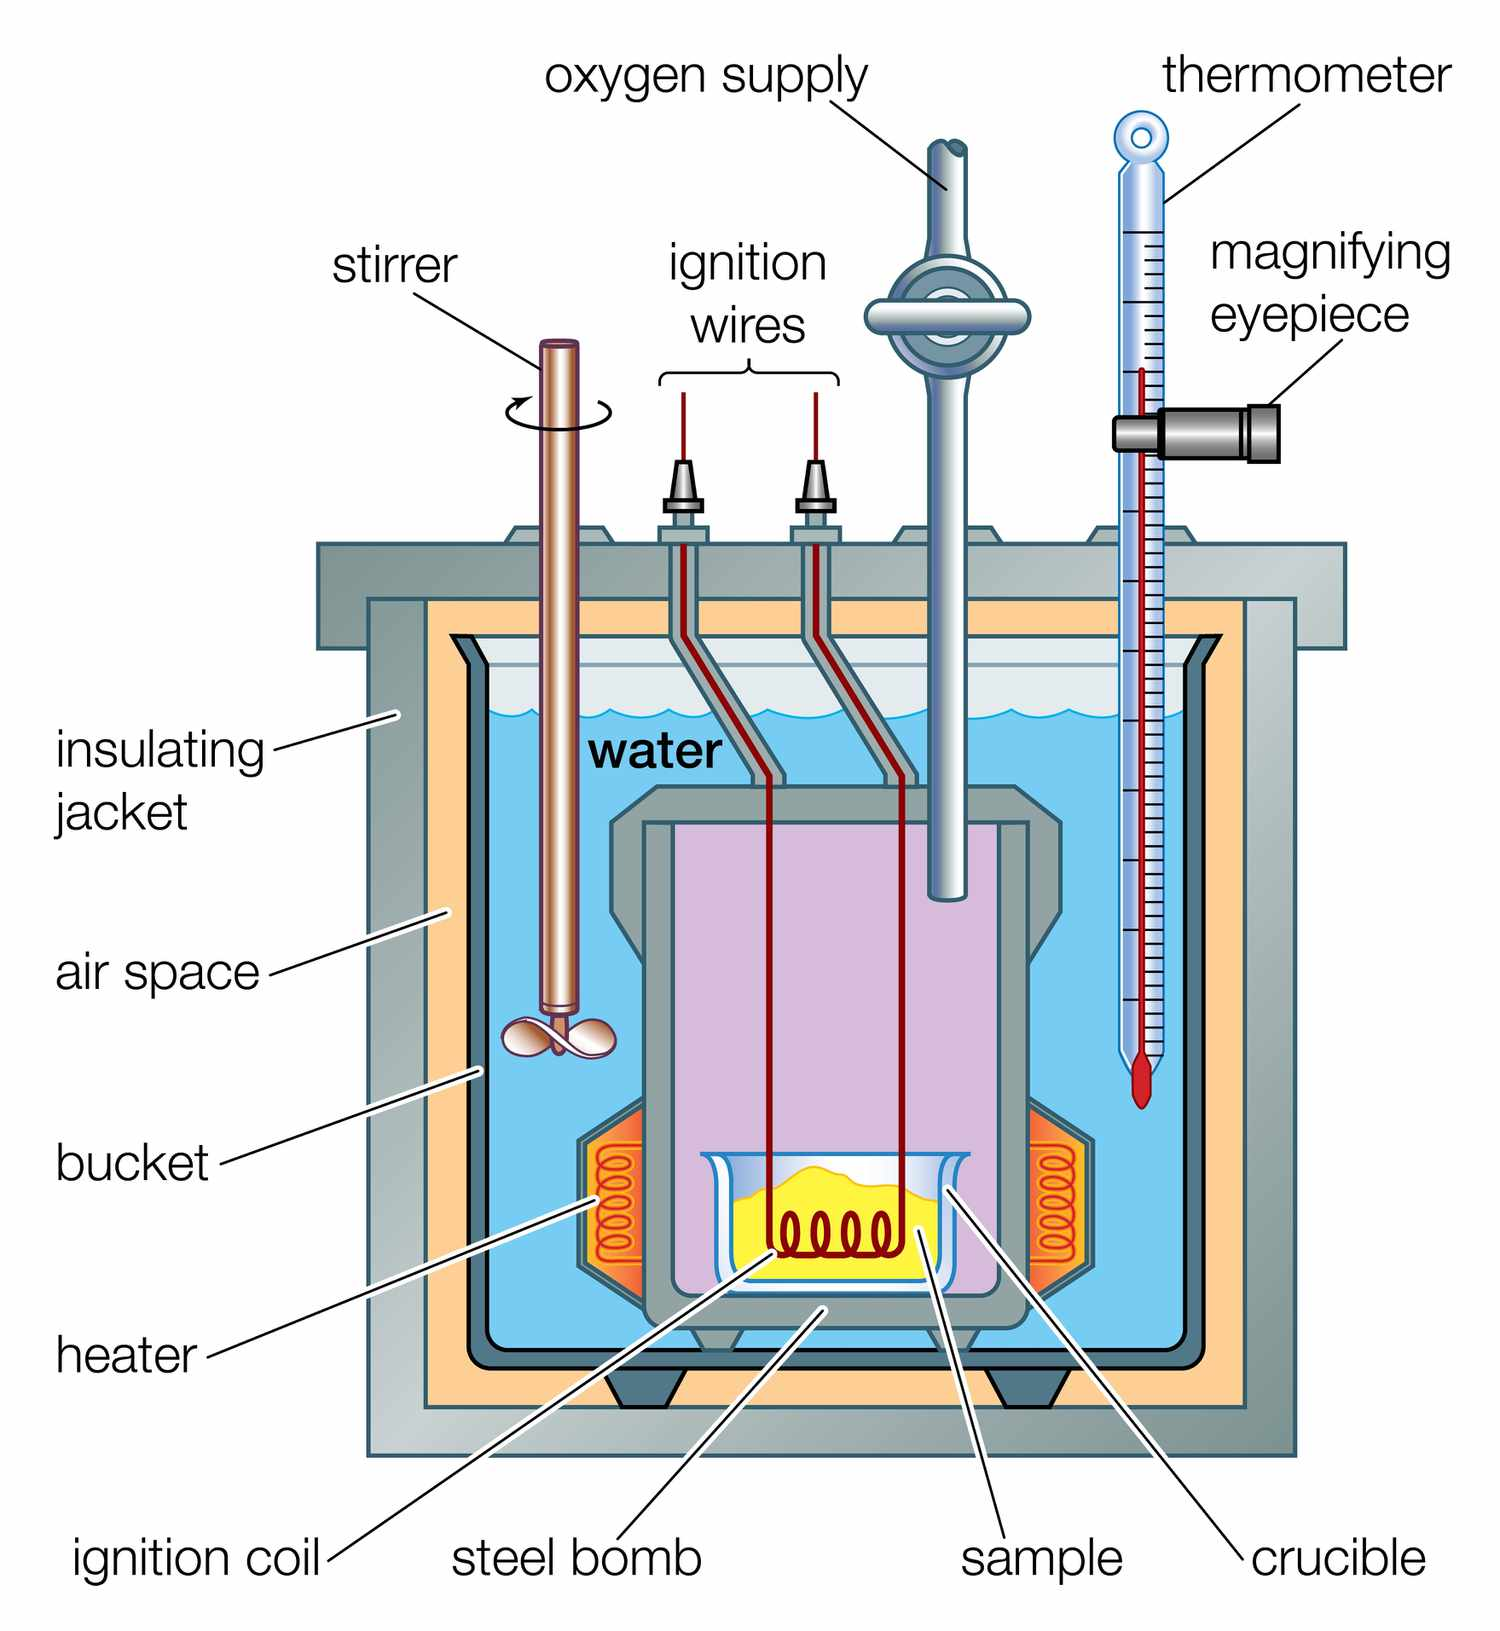
\includegraphics[scale=0.15]{images/bombcal.jpg}
    \caption{A Typical Bomb Calorimeter (\cite{calorimetry})}
    \label{fig:bombcalorimeter}
\end{figure}
\FloatBarrier

\noindent The heat released by an object, $q$, is given by
\begin{equation}\label{eq:heatdefinition}
    q = m \cdot c_p \cdot \Delta T
\end{equation}
\noindent Where $m$ is the mass of the object in grams, $c_p$ is the specific heat capacity, and $\Delta T$ is the change in temperature in kelvin\footnote{The computation is identical if using celcius instead of kelvin, but it is more correct and conventional to use kelvin}. In a bomb calorimeter, little to no heat is lost to the environment, so an analogous statement to the first law of thermodynamics can be stated, that
\begin{gather*}
    q_{c} = -q_{H_2 O}
\end{gather*}
\noindent This suggests that the heat lost by the water ($q_{H_2O}$) is equal to the heat gained by the MNP candidate ($q_c$), and substituting the full expression for heat in \textbf{Eq \ref{eq:heatdefinition}} along with the known specific heat of water, which is $4.18 \frac{J}{g \cdot K}$ yields the following expression for the specific heat of the candidate:
\begin{gather*}
m_c \cdot c_p \cdot \Delta T_c = -m_{H_2O} \cdot (4.18) \cdot \Delta T_{H_2O}
\end{gather*}
\noindent When the candidate is submerged in water, both solute and solvent will reach thermal equilibrium, so the final temperature $T_f$ will be equal for both. Hence, the expression can be expanded:
\begin{gather*}
    \therefore m_c \cdot c_p \cdot (T_f - T_c)) = -m_{H_2O} \cdot (4.18) \cdot (T_f - T_{H_2O}) 
\end{gather*}
Where $T_c$ is the initial temperature of the candidate and $T_{H_2O}$ is the initial temperature of the water before combining both. Finally, we can solve for the specific heat, which is:
\begin{gather*}
       c_p  = -\frac{m_{H_2O} \cdot (4.18) \cdot(T_f - T_{H_2O})} {m_c \cdot (T_f - T_c)}
\end{gather*}
For Iron Oxide, the computation went as follows based on the measured final temperature after 5 minutes, which was 89.44 degrees celsius: 
\begin{gather*}
       c_p  = -\frac{(1.0 \times 10^3) \cdot (4.18) \cdot(89.44 - 90.00)} {0.050 \cdot (89.44 - 20.00)} = 0.67
\end{gather*}
The rest of the candidates were identified in the same way, resulting in the following values (\cite{specificheatinfo}):
\FloatBarrier
\begin{table}[h!]
    \centering
    \begin{tabular}{|c|c|c|} \hline 
      Candidate & Experimental $C_p$  & Established $C_p$ \\ \hline 
      \ce{Fe3O4} &  0.67 & 0.6-0.7\\ \hline 
  \ce{CoFe2O4}    &  0.65 & 0.6-0.7\\ \hline 
   \ce{NiFe2O4}   &  0.64 & 0.6-0.7\\ \hline 
   \ce{MnFe2O4}   & 0.61  & 0.6-0.7\\ \hline 
  \ce{Gd}    & 0.22  & 0.2-0.25
     \\ \hline\end{tabular}
    \caption{Experimental vs Established Values for Each MNP Candidate}
    \label{tab:MNPheatstable}
\end{table}
\noindent All of the computed values are valid, providing some context for the hypothesis: In the context of induced hyperthermia treatment using magnetic nanoparticles, Iron Oxide will likely provide the most heat at all frequencies, while Galodinium should provide the most focused heat at all frequencies, albeit the least. This is because the specific heat capacity of the latter material is very low, meaning it conducts heat easily and directly to the environment compared to Iron Oxide. However, the smaller size of the Galodinium and its dependency on relaxation mechanisms, unlike the hysteresis employed by iron oxide, results in much lower energy efficiency and heat production.

\section{Procedure}
{\textbf{Dependent  Variable(s):} Two quantities will be the focus of the experiment(s): specific absorption rate (SAR) and the area of heat diffusion, a region that I will define as above 37 degrees Celsius (slightly above normal body temperature).\\
\textbf{Independent  Variable:} For the two quantities SAR and Area (dependent variables), the independent variable will be the frequency at which the external alternating magnetic field oscillates.\\
\textbf{Control  Variables:}
Throughout the experiment(s), the molarity of solution containing MNPs and solution fluid (0.5 \textit{M}), initial temperature (20 Degrees Celcius), tumor type and sample mass (1 g), and exposure duration (2 minutes) will remain constant. } There will be 5 data groups for comparison: the aforementioned MNP candidates. Two conjoined experiments will be run using the same sample, and are described below:
\subsection{Experiment 1: SAR}
\textbf{Materials:}
\begin{itemize}
    \item Magnetic Nanoparticle (MNP) Samples: {At least 6 samples of at least 0.05g quantities of each of the 5 candidates discussed above (to maintain constant molarity, candidates with smaller molar masses should have smaller sample sizes), all preferably taken from the same initial sample to maintain purity assumptions.}
    \item AMF Generator: A device capable of generating alternating magnetic fields at various frequencies and field strengths. {It should contain the general low-frequency band (100-1000 kHz).}
    \item Calorimeter: To measure the temperature change of the MNPs, able to hold a volume above 2.5 Liters
    \item Thermometer or Thermocouple: To accurately measure temperature changes.
    \item Water Bath: To maintain a constant initial temperature for all samples.
    \item {Weighing Scale: To measure the mass of the tumor samples}
    \item {Graduated Cylinder: For measuring the volume of fluid}
    \item Insulated Container: To minimize heat loss to the environment, with a volume of at least 2.5 Liters
    \item Magnetic Field Meter: To measure the strength of the magnetic field
    \item Stopwatch or Timer: For timing of the experiment.
    \item Carrier Fluid: In order to mimic human conditions,{ 15 samples of intracellular fluid diluted with water to 0.1 Liters is sufficient}
\end{itemize}
The AMF Generator I used had an integrated stopwatch and magnetic field meter, but for alternative ones, they must be used separately. The methodology is as follows:
\begin{enumerate}
    \item Prepare MNP suspensions in the carrier fluid (like water) at a known concentration, in this case, 0.5$M$. The molarity itself is not important but must be held constant throughout.
    \item Place each MNP suspension in the calorimeter, ensuring a consistent volume for each sample.
    \item Equilibrate all samples to 20 degrees Celsius.
    \item Expose each sample to an AMF at a specific frequency and measure the temperature rise over a fixed interval of 2 minutes.
    \item Record the maximum temperature reached by each sample.
    \item Calculate the SAR using the formula: 
    \begin{equation}
         SAR = (c_{f} \cdot \Delta T \cdot V_f) / (m_c × \Delta t)
    \end{equation}
    where $c_f$ is the specific heat capacity of the carrier fluid, $\Delta T$ is the temperature change, $V$ is the volume of the fluid, $m_c$ is the mass of the MNPs, and $\Delta t$ is the time interval.
    \item Repeat the experiment for different frequencies of the AMF, following 100 kHz, 200 kHz, 300 kHz, up to 1000 kHz, for each candidate, using a new volume of fluid for each.
\end{enumerate}
\subsection{Experiment 2: Area of Heat Diffusion}
\textbf{Materials:}
\begin{itemize}
    \item The same MNP samples, fluid, and AMF generator as in Experiment 1.
    \item Infrared Camera or Thermal Imaging System: To visualize and measure temperature distribution.
    \item 15 cancerous tissue samples of \footnote{Sodium Polyacrylate or another substitute to transform the fluid into a more gel-like phase and mimic tumor tissue is also possible} from a singular tumor, 1g each. In this case, it is an Astrocytoma, a type of malignant brain tumor.
    \item Precision Injection Equipment: For embedding MNPs into the tissue.
    \item Ruler or Caliper: For measuring the heated region.
\end{itemize}
\textbf{Methodology:}
\begin{enumerate}
    \item Embed a known quantity of each MNP (0.01g) type into 5 separate sections of the tumor sample.
    \item Expose the gel to an AMF at a specific frequency.
    \item Use the thermal imaging system to monitor and record the temperature distribution. Only observe the region that is above 37 degrees Celsius around the candidate and measure the smallest and largest radii of this generally circular region.
    \item The average of the smallest and largest radii of heat distribution should be recorded for heat distribution. This can be substituted into the formula for an area of a circle to approximate the heated area.
    \item Repeat the experiment for different frequencies of the AMF and 5 candidates.
\end{enumerate}
\section{Risk Assessment}
\subsection{Safety}
{This experiment was largely carried out within the Trinity Clinical Laboratory in order to access industrial-grade equipment and maintain safety protocol. While working with a powerful alternating magnetic field, similar to general practice around an MRI, no personal belongings were brought near the equipment and all metallic tools used -particularly the stirring rod- were demagnetized prior to use. Gloves, goggles, and laboratory clothing were worn throughout to prevent exposure to heated liquid and prevent burns or contact with contaminants, and masks alongside constant external ventilation were used to prevent the inhalation of contaminants caused by the superheating of the samples. }
\subsection{Ethics}
{All biological samples, namely the tumor samples and intracellular fluid, were sourced responsibly and ethically from donations to Trinity Clinical Laboratories. Aside from the sourcing of materials, there are no other ethical concerns.}
\subsection{Environmental Impact}
{ The amount of either material was minimized but could not be recycled or reused after use due to damage to the tumor from prolonged heat exposure and contamination of the intracellular fluid by magnetic nanoparticles. All materials were disposed of responsibly through the laboratory's waste facilities. The timing was also minimized for stabilizing each frequency band during experimentation to conserve power usage by the AMF generator, though it still remained powered for a considerable amount of time.}

\section{Processed Data}
\textbf{Table \ref{table:data}} contains the averages of the three trials in the appendix for each candidate's specific absorption rate. The following graph is a visual representation. \textbf{Table \ref{table:heat_diffusion}} contains the averages of the three trials for the sufficiently heated area, and it is followed by a graph for visual representation as well (\cite{ChatGPT}).
\subsection{Sample Calculations}
{The following sample calculation is shown for the calculation of SAR (Specific Absorption Rate) for Iron Oxide at the 100 kHz band, seen in} \textbf{Table \ref{table:area_data_trial1}} for the first trial {in the appendix. The equation for SAR is given in Equation 2.1:}
\begin{gather*}
    SAR = (0.67 \cdot ( 23.95 - 20.00) \cdot 0.5) / ((0.05 \times 10 ^{-3}) \cdot 120.0)\\
    = 220.68
\end{gather*}
In the calculation above, the mass of Iron Oxide is converted to kilograms and the time interval to seconds. The final temperature measured was 23.95 degrees Celsius, as seen in the substitution and calculation.\\
{The second sample calculation is used to demonstrate the calculation of the mean for the data in \textbf{Table 2}. Specifically, this calculation is for the calculation of Iron Oxide's SAR at the 100 kHz band as well, using data from \textbf{Tables 5-7}}:
\begin{equation}
    Mean = \frac{1}{n} \times \sum_{i=1}^n T_i
\end{equation}
{Where $T_i$ is the specific data value for the $i$th trial, and $n$ is the total number of trials. In this case, there are 3 trials with values 220.68, 219.86, 220.42 and for the SAR. Therefore,}
\begin{gather*}
   Mean = \frac{1}{3} \times (220.68 + 219.86 + 220.42)\\
   = 220.32
\end{gather*}

\FloatBarrier
{\begin{table}[h]
\centering
\begin{tabular}{|c|c|c|c|c|c|}
\hline
Frequency (kHz $\pm 0.001$) & \ce{Fe3O4}  & \ce{CoFe2O4}  & \ce{NiFe2O4}  & \ce{MnFe2O4}   & \ce{Gd}  \\
\hline
$100.000$ & $220.32  $ &205&190& $185.0$ & 180.01 \\
$200.000$&$198.05$&$183.12$ & $166.05  $ & $159.31  $ & $152.15  $ \\
$300.000$ & $220.33  $ & 205.01 & $196.06  $ & $185.12  $ & $181.73  $ \\
$400.000$ & $242.12  $ & $227.01$ & $200.88  $ & $210.22  $ & $200.76  $ \\
$500.000$ & $218.01  $ & $205.00$ & $193.01$ & $185.00$ & $180.01$ \\
$600.000$ & $198.12  $ & $180.33  $ & $160.45  $ & $159.01$ & $152.00$ \\
$700.000$ & $223.01  $ & $204.89  $ & $186.87  $ & $185.32  $ & $180.19  $ \\
$800.000$ & $242.12  $ & $227.32  $ & $214.18  $ & $213.32  $ & $209.76  $ \\
$900.000$ & $220.22  $ & $203.66  $ & $191.32  $ & $185.21  $ & $182.76  $ \\
$1000.000$ & $198.02  $ & $183.77  $ & $176.99  $ & $159.64  $ & $152.06  $ \\
\hline
\end{tabular}
\caption{Heat production (SAR $\pm 0.01$) vs frequency (kHz $\pm 0.001$) (avg of \textbf{Table \ref{table:area_data_trial1}, \ref{table:area_data_trial2}, \ref{table:area_data_trial3}})}
\label{table:data}
\end{table}}
\FloatBarrier
\begin{figure}[h!]
    \centering
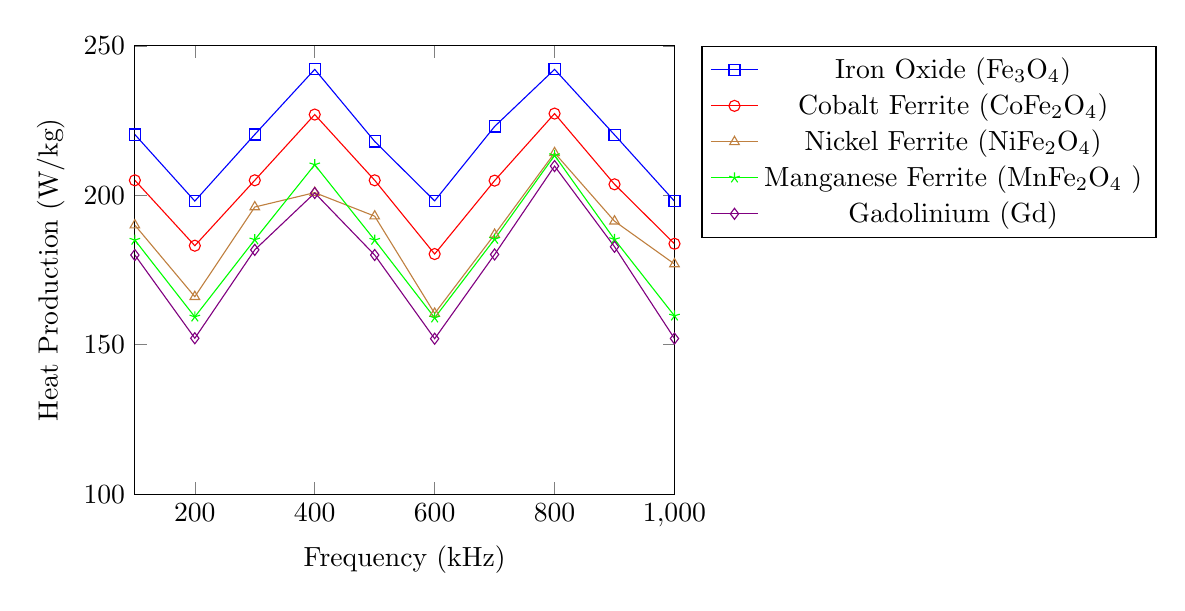
\begin{tikzpicture}
\begin{axis}[
    xlabel={Frequency (kHz)},
    ylabel={Heat Production (W/kg)},
    xmin=100, xmax=1000,
    ymin=100, ymax=250,
    legend style={at={(1.05,1)}, anchor=north west},
    grid style=dashed,
]

\addplot[color=blue, mark=square] coordinates {
    (100,220.32)(200,198.05)(300,220.33)(400,242.12)(500,218.01)(600,198.12)(700,223.01)(800,242.12)(900,220.22)(1000,198.02)
};
\addlegendentry{Iron Oxide (\ce{Fe3O4})}

\addplot[color=red, mark=o] coordinates {
    (100,205)(200,183.12)(300,205)(400,227)(500,205)(600,180.33)(700,204.89)(800,227.32)(900,203.66)(1000,183.77)
};
\addlegendentry{Cobalt Ferrite (\ce{CoFe2O4})}

\addplot[color=brown, mark=triangle] coordinates {
    (100,190)(200,166.05)(300,196.06)(400,200.88)(500,193)(600,160.45)(700,186.87)(800,214.18)(900,191.32)(1000,176.99)
};
\addlegendentry{Nickel Ferrite (\ce{NiFe2O4})}

\addplot[color=green, mark=star] coordinates {
    (100,185.0)(200,159.31)(300,185.12)(400,210.22)(500,185)(600,159)(700,185.32)(800,213.32)(900,185.21)(1000,159.64)
};
\addlegendentry{Manganese Ferrite (\ce{MnFe2O4} )}

\addplot[color=violet, mark=diamond] coordinates {
    (100,180)(200,152.15)(300,181.73)(400,200.76)(500,180)(600,152)(700,180.19)(800,209.76)(900,182.76)(1000,152.06)
};
\addlegendentry{Gadolinium (\ce{Gd})}

\end{axis}
\end{tikzpicture}
    \caption{Heat production (SAR $\pm 0.01$) vs frequency (kHz $\pm 0.001$) (Data from \textbf{Table \ref{table:data}})}
    \label{fig:graphheatall}
\end{figure}

\FloatBarrier
\begin{table}[h]
\centering
\begin{tabular}{|c|c|c|c|c|c|}
\hline
Frequency (kHz $\pm 0.001$) & {\ce{Fe3O4}}  & \ce{CoFe2O4} & {\ce{NiFe2O4}}  & {\ce{MnFe2O4} }  & \ce{Gd}   \\
\hline
100.000 & 45.4 & 43.2 & 41.4 & 39.6 & 37.8 \\
200.000  & 40.6 & 38.4 & 36.8 & 35.2 & 33.6 \\
300.000  & 35.7 & 33.6 & 32.2 & 30.8 & 29.4 \\
400.000  & 30.2 & 28.8 & 27.6 & 26.4 & 25.2 \\
500.000  & 25.1 & 24.3 & 23.2 & 22.1 & 21.6 \\
600.000  & 20.4 & 19.2 & 18.4 & 17.6 & 16.8 \\
700.000  & 15.2 & 14.4 & 13.8 & 13.2 & 12.6 \\
800.000  & 10.3 & 9.6 & 9.2 & 8.8 & 8.4 \\
900.000  & 5.3 & 4.8 & 4.6 & 4.4 & 4.2 \\
1000.000  & $\sim0$ & 2.1 & 2.1 & 2.1 & 2.0 \\
1100.000  & $\sim0$ & $\sim0$ & $\sim0$ & $\sim0$ & $\sim 0$ \\
\hline
\end{tabular}
\caption{Area of heat diffusion (mm$^2 \pm 0.1$ ) vs frequency (kHz $\pm 0.001$) (avg of \textbf{Table \ref{table:heat_data_trial1}, \ref{table:heat_data_trial2}, \ref{table:heat_data_trial3}})}
\label{table:heat_diffusion}
\end{table}
\FloatBarrier
\begin{figure}[h!]
    \centering
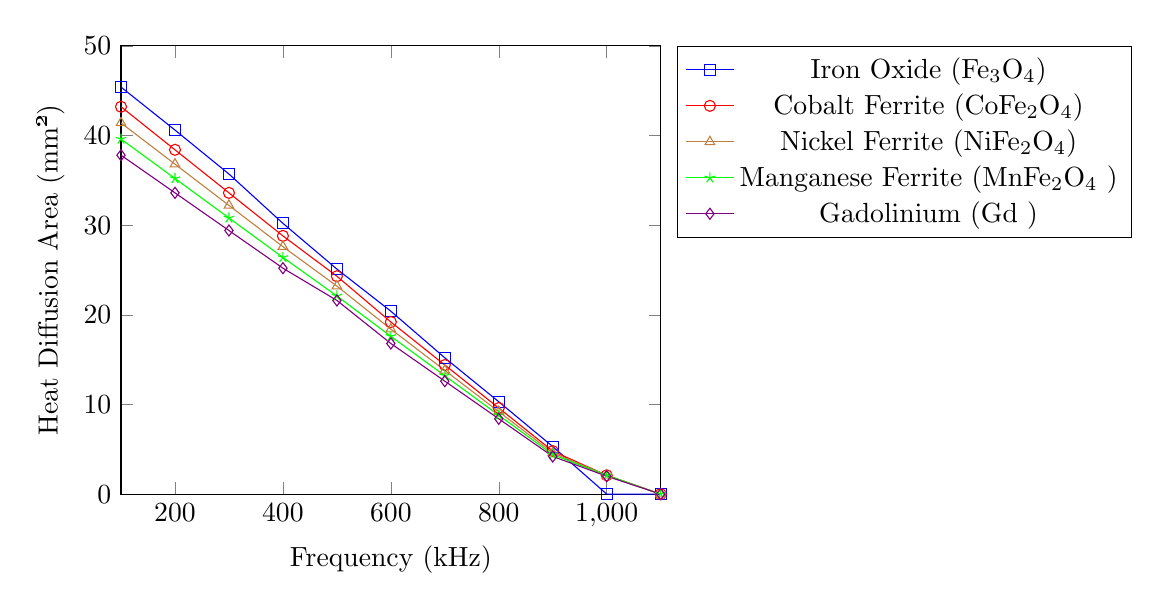
\begin{tikzpicture}
\begin{axis}[
    xlabel={Frequency (kHz)},
    ylabel={Heat Diffusion Area (mm²)},
    xmin=100, xmax=1100,
    ymin=0, ymax=50,
    legend pos=outer north east,
    grid style=dashed,
]
\addplot[color=blue, mark=square,] coordinates {
    (100,45.4)(200,40.6)(300,35.7)(400,30.2)(500,25.1)(600,20.4)(700,15.2)(800,10.3)(900,5.3)(1000,0)(1100,0)
};
\addplot[color=red, mark=o,] coordinates {
    (100,43.2)(200,38.4)(300,33.6)(400,28.8)(500,24.3)(600,19.2)(700,14.4)(800,9.6)(900,4.8)(1000,2.1)(1100,0)
};
\addplot[color=brown, mark=triangle,] coordinates {
    (100,41.4)(200,36.8)(300,32.2)(400,27.6)(500,23.2)(600,18.4)(700,13.8)(800,9.2)(900,4.6)(1000,2.1)(1100,0)
};
\addplot[color=green, mark=star,] coordinates {
    (100,39.6)(200,35.2)(300,30.8)(400,26.4)(500,22.1)(600,17.6)(700,13.2)(800,8.8)(900,4.4)(1000,2.1)(1100,0)
};
\addplot[color=violet, mark=diamond,] coordinates {
    (100,37.8)(200,33.6)(300,29.4)(400,25.2)(500,21.6)(600,16.8)(700,12.6)(800,8.4)(900,4.2)(1000,2.0)(1100,0)
};
\legend{Iron Oxide (\ce{Fe3O4}), Cobalt Ferrite (\ce{CoFe2O4}), Nickel Ferrite (\ce{NiFe2O4}), Manganese Ferrite (\ce{MnFe2O4} ), Gadolinium (\ce{Gd} )}
\end{axis}
\end{tikzpicture}
    \caption{Heat Diffusion Area (mm$^2 \pm 0.1$) vs Frequency (kHz $\pm 0.001$) (Data from \textbf{Table \ref{table:heat_diffusion}})}
    \label{fig:graphdiffusionarea}
\end{figure}
\FloatBarrier
\section{Data Analysis and Conclusion}
The individual graphs that make both \textbf{Figure \ref{fig:graphheatall}, \ref{fig:graphdiffusionarea}} are presented in the appendix, though the error bars have been omitted as they are too small to see for the graphs' scale. For the respective graphs of heated area, the following $R^2$ values were computed using \textbf{Wolfram Alpha} (\cite{wolframalpha}):
\FloatBarrier
\begin{table}[h!]
    \centering
    \begin{tabular}{|c|c|} \hline 
        \ce{Fe3O4} &  0.9935\\ \hline 
        \ce{CoFe2O4} & 0.9940 \\ \hline 
        \ce{NiFe2O4} & 0.9940 \\ \hline 
        \ce{MnFe2O4} &  0.9939\\ \hline 
        \ce{Gd}   &  0.9939
     \\ \hline\end{tabular}
    \caption{$R^2$ Values For Heated Areas}
    \label{tab:R2values}
\end{table}
\FloatBarrier
\noindent The $R_2$ values are very close to 1, indicating a strong linear trend and suggesting that the data for the area of heat dispersion is reliable. {The graph for SAR vs. frequency was not able to be statistically evaluated using this method as a suitable best-fit function -which would most likely be sinusoidal- could not be determined. As a result, qualitative observation was necessary for analysis.} Based on both graphs above, it is evident that Iron Oxide seems to be the best candidate for hyperthermia treatment for larger tumors, due to its high heat output alongside a larger region of increased heat. Meanwhile, a candidate like Gadolinium is a better candidate for smaller tumors located in "riskier" areas near or within vital organs, where there is little to no room for error, justified by comparing the data in \textbf{Tables \ref{fig:feheatgeneration}, \ref{fig:gdheatgeneration}} and \textbf{Tables \ref{fig:fearea}}, \ref{fig:gdarea} respectively. As for the candidates in between, they may offer use in specialized cases where a balance of both size and heat generation is necessary, but a more quantitative comparison cannot be drawn reliably. All candidates, however, produced sufficient heat to at least begin apoptosis in cancerous cells. \\
{In conclusion, the results of this investigation fall in line with the preceding scientific literature on MNP candidates for hyperthermia treatment, supporting my hypothesis strongly. Iron Oxide has been established as an ideal candidate for hyperthermia treatment by} \cite{JIANG2022107707}, {which is agreed upon by this investigation. Clear relationships are distinguished and supported by the theoretical framework put forth by the medical physicists who pioneered this method. Many medical physics studies have treated iron oxide as the ideal candidate for this treatment. However, none I found online offered concrete evidence for its effectiveness} (\cite{JIANG2022107707}). However, few had mentioned Gadolinium, which is likely a result of its relatively new appearance in the realm of medical physics as a biocompatible medium. In fact, hyperthermia as a whole was a relatively unknown treatment when researching online for supplementary theoretical information, but the conclusions drawn from this experiment suggest the importance of continuing research.

\subsection{Strengths}
The instrumental uncertainties in my data were low enough to a point where they could be ignored, as they were invisible graphically {- a merit of having access to laboratory equipment for this experiment. Particularly, the temperature probes used were very precise compared to the standard vernier lab quest I had initially intended to use, resulting in negligible error bars. Another strength was the purity of samples available, evinced by the alignment of their experimental specific heat capacities with the generally established values. This led to a linear and proportional trend in the heat diffusion vs. frequency of the alternating magnetic field. A final strength was the numerous availability of fluid and tumor samples for the experiment that allowed for using new, uncontaminated samples for each trial leading to minimized random error.}


\subsection{Limitations}
{ Discussing limitations, in }\textbf{Figure \ref{fig:graphdiffusionarea}}, {the linearity of all candidates seems to crumble near the 1000 kHz mark. However, this still remains within the low band of frequencies, suggesting an issue with the equipment I used, as the AMF generator may have had issues maintaining such high frequencies for prolonged periods of time, as it was only meant to produce 1000 kHz for about 30 seconds, which may have led to damage.} This was evinced by the heat dispersion changing rapidly over time during the trials for Nickel Ferrite -which took place near the end of the experimentation period, leading to significantly more different raw data in the 3 trials for this candidate than others and a deviation from the general oscillating trend seen in \textbf{Figure \ref{fig:graphheatall}}. \\
{Furthermore, another potential source of error that I had initially failed to consider was the implications that an alternating magnetic field had on the established charge gradient of cells in the affected region. For cells that make use of electrochemical gradients -evinced by the usage of sodium-potassium pumps- for homeostasis, this magnetic field could disrupt their equilibrium by its force exerted on the charged particles, as it causes them to move more randomly and less in the direction of the diffusion facilitated by active transport, creating an imbalance in the cell's potential gradient.} While this effect is negligible in the context of survival rates, the resulting shift in the electrochemical gradient of the MNPs' surroundings could lead to deviation in the measured heat diffusion areas in \textbf{Table \ref{table:heat_diffusion}}, due to the increased interactions of the MNPs with charged particles, as more background medium will have increased kinetic energy. {As a result, the model used to measure heat dispersion becomes more approximate than I initially expected - another limitation.}\\

\subsection{Improvements and Extensions}
{The experimental methodologies in this exploration can be improved by using larger volumes of intracellular fluid to minimize uncertainty regarding the molarity of the solution - though it was considered negligible in the first place. Another improvement would result from using a more specialized fluid similar to the delivery agent used with MNPs in standard hyperthermia treatment, which was unavailable in quantities sufficient for the experiment at the time of experimentation} (\cite{immune}). {More precise equipment can always be used, and more specifically, rather than a standard water bath, an industrial-grade circulating bath would be far more efficient in energy consumption and the precision of temperature. The experiment could not use a bath designed specifically for intracellular fluid, so a water bath was used. Any method of reusing the fluid by separating the MNPs from the solution would greatly increase the efficiency of the experiment, but such a method was not found throughout the course of the experiment.}
 {Continuing research will consist of experimentation across a wide variety of tumor tissues to see if the same candidates hold the most value in specific cases, or if certain, unknown physical/chemical properties of these candidates will affect their viability. Identifying these properties is something that would greatly increase the validity of information in my experiment, as these properties had seemingly profound impacts on the viability of candidates yet were unable to be determined by the resources I had available. Furthermore, using another AMF that is not restricted to the low-frequency band can provide further insight into the sinusoidal pattern that emerges from the SAR vs Frequency Graph - verifying if this pattern continues past the low-frequency band. Finally, the exploration of more candidates will always be a viable option for further research, and which candidates should be chosen can be more well understood by the aforementioned research on the role chemical properties play in the relaxation mechanisms of magnetic nanoparticles.}

\newpage
\section{Appendix}
The following \textbf{Tables \ref{table:area_data_trial1}, \ref{table:area_data_trial2}, \ref{table:area_data_trial3}} were the collected measurements for the amount of heat produced by each MNP candidate in 3 trials. The instrumental uncertainty for each candidate's heat measurements was $\pm 0.01 \, \text{W/kg or SAR}$.
\begin{table}[h!]
\centering
\begin{tabular}{|c|c|c|c|c|c|}
\hline
Frequency (kHz $\pm 0.001$) & \ce{Fe3O4} & \ce{CoFe2O4} & \ce{NiFe2O4} & \ce{MnFe2O4}  & \ce{Gd}  \\
\hline
$100.000$ & 220.68 & 205.76 & 189.73 & 185.48 & 180.46 \\
$200.000$ & 197.55 & 183.22 & 166.51 & 161.03 & 151.58 \\
$300.000 $ & 220.74 & 205.94 & 196.91 & 185.88 & 181.96 \\
$400.000$ & 242.01 & 226.19 & 201.26 & 212.04 & 201.96 \\
$500.000 $ & 217.60 & 203.98 & 192.45 & 184.91 & 180.03 \\
$600.000$ & 197.20 & 181.17 & 162.06 & 158.91 & 151.77 \\
$700.000$ & 223.40 & 205.70 & 187.02 & 184.78 & 181.53 \\
$800.000$ & 242.41 & 227.88 & 214.41 & 212.48 & 209.47 \\
$900.000$ & 220.43 & 202.94 & 191.24 & 184.83 & 181.46 \\
$1000.000$ & 198.12 & 183.61 & 176.36 & 159.55 & 151.79 \\
\hline
\end{tabular}
\caption{Heat production (SAR $\pm 0.001$) vs frequency (kHz $\pm 0.001$) for candidates (Trial 1)}
\label{table:area_data_trial1}
\end{table}

\begin{table}[h!]
\centering
\begin{tabular}{|c|c|c|c|c|c|}
\hline
Frequency (kHz $\pm 0.001$) & \ce{Fe3O4}  & \ce{CoFe2O4}  & \ce{NiFe2O4}  & \ce{MnFe2O4}   & \ce{Gd}  \\
\hline
$100.000$ & 219.86 & 204.21 & 191.24 & 184.54 & 180.89 \\
$200.000$ & 197.63 & 182.83 & 165.87 & 158.48 & 152.19 \\
$300.000$ & 219.78 & 204.64 & 195.17 & 183.41 & 181.04 \\
$400.000$ & 241.53 & 226.28 & 199.92 & 209.27 & 200.13 \\
$500.000$ & 217.79 & 205.41 & 193.86 & 185.02 & 180.73 \\
$600.000$ & 198.88 & 179.06 & 159.78 & 159.15 & 152.43 \\
$700.000$ & 223.46 & 205.01 & 187.24 & 186.59 & 179.56 \\
$800.000$ & 240.92 & 226.03 & 214.25 & 213.98 & 210.64 \\
$900.000$ & 220.97 & 205.31 & 191.78 & 185.06 & 183.26 \\
$1000.000$ & 198.34 & 183.52 & 178.20 & 159.37 & 152.23 \\
\hline
\end{tabular}
\caption{Heat production (SAR $\pm 0.01$) vs frequency (kHz $\pm 0.001$) for candidates (Trial 2)}
\label{table:area_data_trial2}
\end{table}

\begin{table}[h!]
\centering
\begin{tabular}{|c|c|c|c|c|c|}
\hline
Frequency (kHz $\pm 0.001$) & \ce{Fe3O4}  & \ce{CoFe2O4}  & \ce{NiFe2O4}  & \ce{MnFe2O4}   & \ce{Gd}  \\
\hline
$100.0$ & 220.42 & 205.04 & 189.03 & 184.98 & 178.64 \\
$200.0$ & 198.97 & 183.31 & 165.77 & 158.42 & 152.69 \\
$300.0$ & 220.47 & 204.42 & 196.10 & 186.07 & 182.19 \\
$400.0$ & 242.81 & 228.52 & 201.47 & 209.35 & 200.19 \\
$500.0$ & 218.64 & 205.61 & 192.69 & 185.07 & 179.24 \\
$600.0$ & 198.28 & 180.76 & 159.51 & 158.94 & 151.79 \\
$700.0$ & 222.17 & 203.97 & 186.35 & 184.59 & 179.48 \\
$800.0$ & 243.03 & 228.05 & 213.88 & 213.50 & 209.17 \\
$900.0$ & 219.26 & 202.73 & 190.94 & 185.74 & 183.57 \\
$1000.0$ & 197.60 & 184.18 & 176.41 & 160.00 & 152.16 \\
\hline
\end{tabular}
\caption{Heat production (SAR $\pm 0.01$) vs frequency (kHz $\pm 0.001$) for candidates (Trial 3)}
\label{table:area_data_trial3}
\end{table}

\FloatBarrier
The following \textbf{Tables \ref{table:heat_data_trial1}, \ref{table:heat_data_trial2}, \ref{table:heat_data_trial3}} were the collected measurements for the area of sufficient heat produced by each MNP candidate in 3 trials. The instrumental uncertainty for each candidate's area measurements was $\pm 0.1 \, \text{mm}^2$.
\FloatBarrier
\begin{table}[h]
\centering
\begin{tabular}{|c|c|c|c|c|c|}
\hline
Frequency (kHz $\pm$ 0.001) & {\ce{Fe3O4}}  & \ce{CoFe2O4} & {\ce{NiFe2O4}}  & {\ce{MnFe2O4} }  & \ce{Gd}   \\
\hline
100.000  & 46.08 & 43.73 & 41.15 & 39.77 & 37.9 \\
200.000  & 40.6 & 37.85 & 37.09 & 34.29 & 34.44 \\
300.000  & 36.1 & 33.59 & 31.09 & 31.56 & 30.49 \\
400.000  & 30.1 & 27.82 & 27.88 & 26.15 & 25.44 \\
500.000  & 25.86 & 25.28 & 22.21 & 22.64 & 22.27 \\
600.000  & 19.42 & 19.24 & 19.17 & 17.79 & 16.16 \\
700.000  & 14.99 & 14.64 & 13.54 & 11.99 & 13.77 \\
800.000  & 9.85 & 10.37 & 8.36 & 9.8 & 7.77 \\
900.000  & 5.6 & 4.87 & 4.95 & 4.73 & 4.13 \\
1000.000  & $\sim0$ & 1.87 & 2.02 & 2.27 & 2.17 \\
1100.000  & $\sim0$ & $\sim0$ & $\sim0$ &$\sim0$ & $\sim0$ \\
\hline
\end{tabular}
\caption{Area of heat diffusion (mm$^2 \pm 0.1$ ) vs frequency (kHz $\pm 0.001$) - Trial 1}
\label{table:heat_data_trial1}
\end{table}
\FloatBarrier
\begin{table}[h]
\centering
\begin{tabular}{|c|c|c|c|c|c|}
\hline
Frequency (kHz $\pm$ 0.001) & {\ce{Fe3O4}}  & \ce{CoFe2O4} & {\ce{NiFe2O4}}  & {\ce{MnFe2O4} }  & \ce{Gd}   \\
\hline
100.000  & 44.88 & 42.88 & 41.62 & 39.3 & 38.2 \\
200.000  & 40.92 & 39.08 & 36.14 & 36.96 & 34.32 \\
300.000  & 35.77 & 34.29 & 32.73 & 29.71 & 29.15 \\
400.000  & 29.93 & 30.17 & 27.89 & 26.58 & 24.24 \\
500.000  & 24.97 & 25.07 & 24.97 & 22.4 & 20.81 \\
600.000  & 20.69 & 18.43 & 18.41 & 17.73 & 17.13 \\
700.000  & 15.59 & 14.11 & 13.39 & 13.59 & 12.15 \\
800.000  & 9.9 & 10.17 & 10.02 & 8.1 & 8.88 \\
900.000  & 4.95 & 4.28 & 4.24 & 4.06 & 4.46 \\
1000.000  & 0 & 2.18 & 2.23 & 2.04 & 1.94 \\
1100.000  & 0 & 0 & 0 & 0 & 0 \\
\hline
\end{tabular}
\caption{Area of heat diffusion (mm$^2 \pm 0.1$ ) vs frequency (kHz $\pm 0.001$) - Trial 2}
\label{table:heat_data_trial2}
\end{table}
\FloatBarrier
\begin{table}[h]
\centering
\begin{tabular}{|c|c|c|c|c|c|}
\hline
Frequency (kHz $\pm$ 0.001) & {\ce{Fe3O4}}  & \ce{CoFe2O4} & {\ce{NiFe2O4}}  & {\ce{MnFe2O4} }  & \ce{Gd}   \\
\hline
100.000  & 45.24 & 42.99 & 41.43 & 39.73 & 37.3 \\
200.000  & 40.28 & 38.26 & 37.17 & 34.35 & 32.04 \\
300.000  & 35.23 & 32.92 & 32.78 & 31.13 & 28.56 \\
400.000  & 30.57 & 28.41 & 27.03 & 26.47 & 25.92 \\
500.000  & 24.47 & 22.55 & 22.42 & 21.26 & 21.72 \\
600.000  & 21.09 & 19.93 & 17.62 & 17.28 & 17.1 \\
700.000  & 15.02 & 14.45 & 14.47 & 14.02 & 11.88 \\
800.000  & 11.14 & 8.27 & 9.22 & 8.49 & 8.55 \\
900.000  & 5.35 & 5.25 & 4.6 & 4.41 & 4.01 \\
1000.000  & 0 & 2.25 & 2.05 & 1.99 & 1.89 \\
1100.000  & 0 & 0 & 0 & 0 & 0 \\
\hline
\end{tabular}
\caption{Area of heat diffusion (mm$^2 \pm 0.1$ ) vs frequency (kHz $\pm 0.001$) - Trial 3}
\label{table:heat_data_trial3}
\end{table}
\FloatBarrier
\subsection{Heat Dispersion Graphs}
\FloatBarrier
\begin{figure}[h!]
    \centering
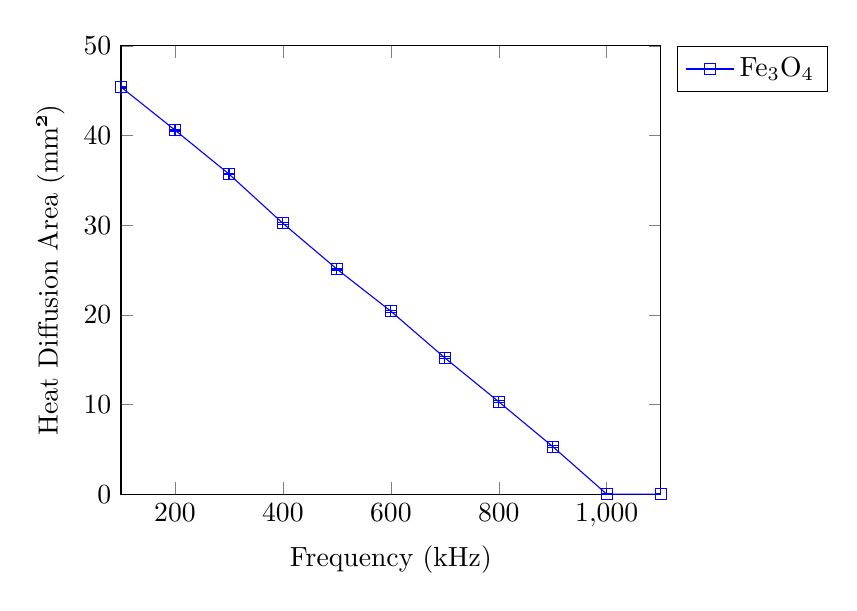
\begin{tikzpicture}
\begin{axis}[
    xlabel={Frequency (kHz)},
    ylabel={Heat Diffusion Area (mm²)},
    xmin=100, xmax=1100,
    ymin=0, ymax=50,
    legend pos=outer north east,
    grid style=dashed,
]

\addplot+[blue, mark=square, error bars/.cd, x dir=both, x fixed=0.001, y dir=both, y fixed=0.1]
coordinates {
    (100,45.4)
    (200,40.6)
    (300,35.7)
    (400,30.2)
    (500,25.1)
    (600,20.4)
    (700,15.2)
    (800,10.3)
    (900,5.3)
    (1000,0)
    (1100,0)
};
\legend{\ce{Fe3O4}} % Update the legend with the actual material name
\end{axis}
\end{tikzpicture}
    \caption{Area of heat diffusion (mm$^2 \pm 0.1$ ) vs frequency (kHz $\pm 0.001$) for \ce{Fe3O4}}
    \label{fig:fearea}
\end{figure}
\FloatBarrier
\begin{figure}[h!]
    \centering
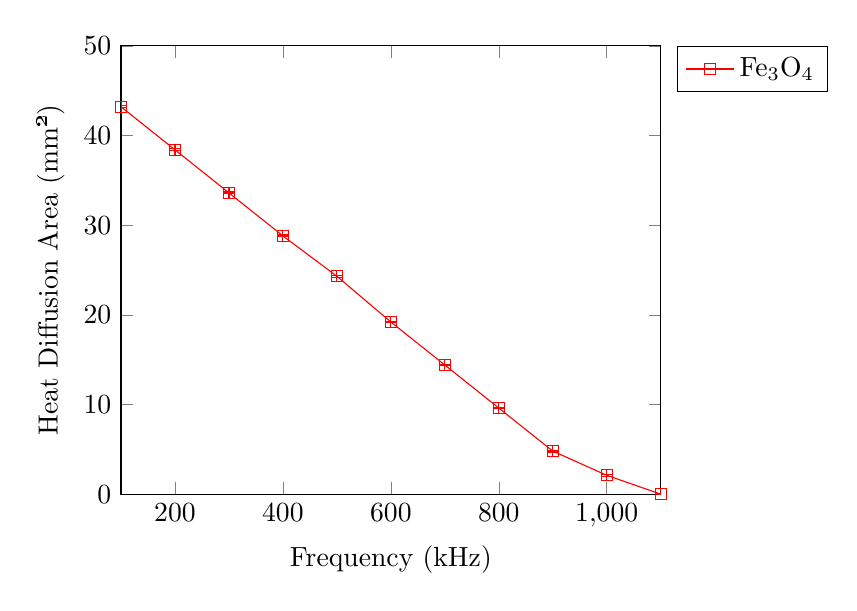
\begin{tikzpicture}
\begin{axis}[
    xlabel={Frequency (kHz)},
    ylabel={Heat Diffusion Area (mm²)},
    xmin=100, xmax=1100,
    ymin=0, ymax=50,
    legend pos=outer north east,
    grid style=dashed,
]

\addplot+[red, mark=square, error bars/.cd, x dir=both, x fixed=0.001, y dir=both, y fixed=0.1]
coordinates {
   (100,43.2)(200,38.4)(300,33.6)(400,28.8)(500,24.3)(600,19.2)(700,14.4)(800,9.6)(900,4.8)(1000,2.1)(1100,0)
};
\legend{\ce{Fe3O4}} % Update the legend with the actual material name
\end{axis}
\end{tikzpicture}
    \caption{Area of heat diffusion (mm$^2 \pm 0.1$ ) vs frequency (kHz $\pm 0.001$) for \ce{CoFe2O4}}
    \label{fig:coarea}
\end{figure}
\FloatBarrier
\begin{figure}[h!]
    \centering
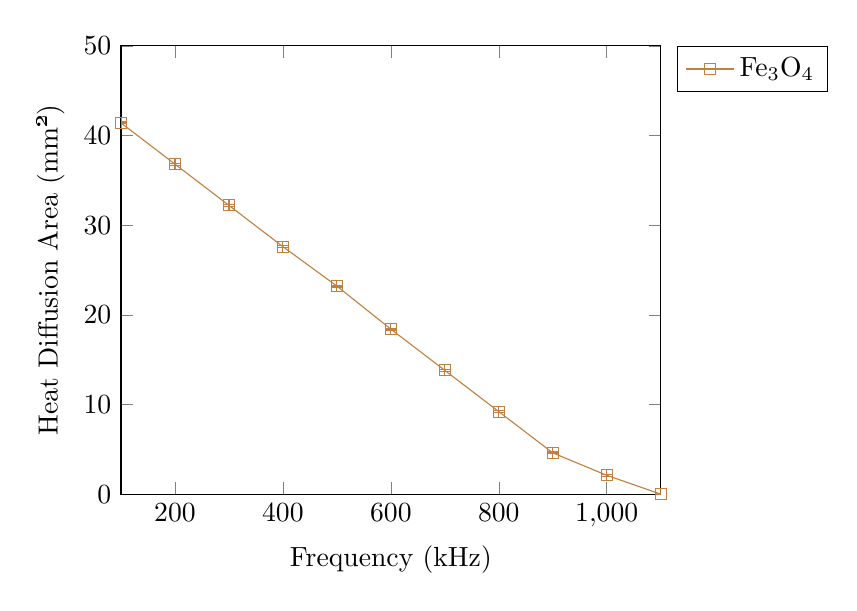
\begin{tikzpicture}
\begin{axis}[
    xlabel={Frequency (kHz)},
    ylabel={Heat Diffusion Area (mm²)},
    xmin=100, xmax=1100,
    ymin=0, ymax=50,
    legend pos=outer north east,
    grid style=dashed,
]

\addplot+[brown, mark=square, error bars/.cd, x dir=both, x fixed=0.001, y dir=both, y fixed=0.1]
coordinates {
    (100,41.4)(200,36.8)(300,32.2)(400,27.6)(500,23.2)(600,18.4)(700,13.8)(800,9.2)(900,4.6)(1000,2.1)(1100,0)
};
\legend{\ce{Fe3O4}} % Update the legend with the actual material name
\end{axis}
\end{tikzpicture}
    \caption{Area of heat diffusion (mm$^2 \pm 0.1$ ) vs frequency (kHz $\pm 0.001$) for \ce{CoNi2O4}}
    \label{fig:niarea}
\end{figure}
\FloatBarrier
\begin{figure}[h!]
    \centering
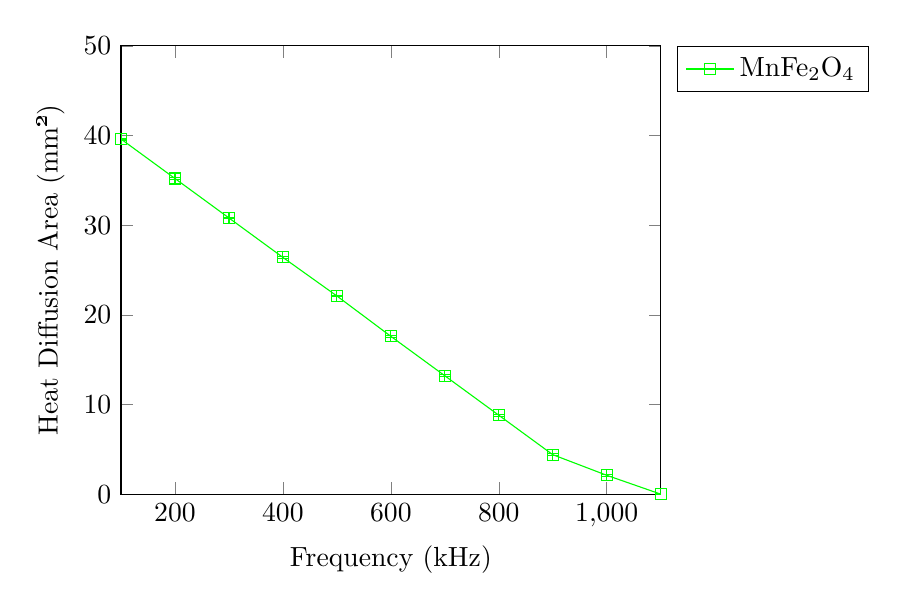
\begin{tikzpicture}
\begin{axis}[
    xlabel={Frequency (kHz)},
    ylabel={Heat Diffusion Area (mm²)},
    xmin=100, xmax=1100,
    ymin=0, ymax=50,
    legend pos=outer north east,
    grid style=dashed,
]

\addplot+[green, mark=square, error bars/.cd, x dir=both, x fixed=0.001, y dir=both, y fixed=0.1]
coordinates {
      (100,39.6)(200,35.2)(300,30.8)(400,26.4)(500,22.1)(600,17.6)(700,13.2)(800,8.8)(900,4.4)(1000,2.1)(1100,0)
};
\legend{\ce{MnFe2O4}} % Update the legend with the actual material name
\end{axis}
\end{tikzpicture}
    \caption{Area of heat diffusion (mm$^2 \pm 0.1$ ) vs frequency (kHz $\pm 0.001$) for \ce{MnFe2O4}}
    \label{fig:mnarea}
\end{figure}
\begin{figure}[h!]
    \centering
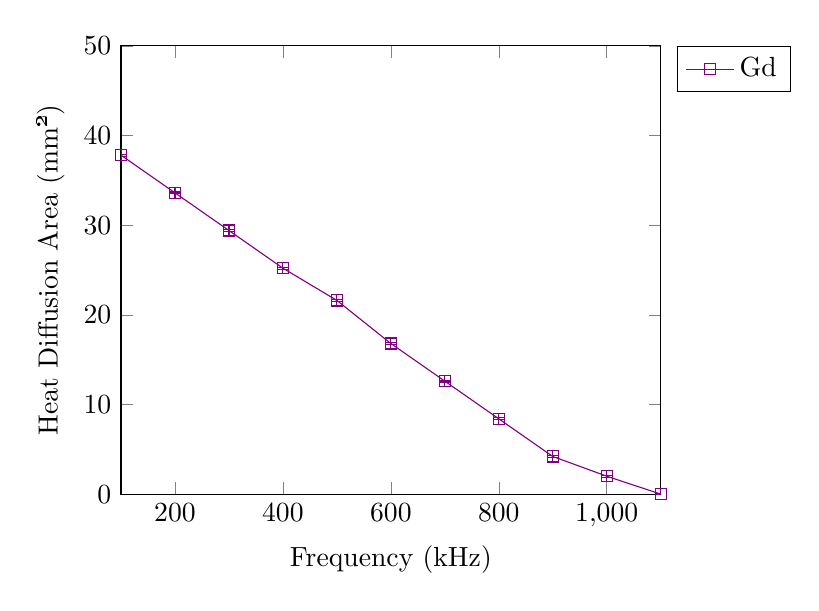
\begin{tikzpicture}
\begin{axis}[
    xlabel={Frequency (kHz)},
    ylabel={Heat Diffusion Area (mm²)},
    xmin=100, xmax=1100,
    ymin=0, ymax=50,
    legend pos=outer north east,
    grid style=dashed,
]

\addplot+[violet, mark=square, error bars/.cd, x dir=both, x fixed=0.001, y dir=both, y fixed=0.1]
coordinates {
(100,37.8)(200,33.6)(300,29.4)(400,25.2)(500,21.6)(600,16.8)(700,12.6)(800,8.4)(900,4.2)(1000,2.0)(1100,0)
};
\legend{\ce{Gd}} % Update the legend with the actual material name
\end{axis}
\end{tikzpicture}
    \caption{Area of heat diffusion (mm$^2 \pm 0.1$ ) vs frequency (kHz $\pm 0.001$) for \ce{Gd}}
    \label{fig:gdarea}
\end{figure}

\FloatBarrier
\subsection{Heat Production Graphs}
\FloatBarrier
\begin{figure}[h!]
    \centering
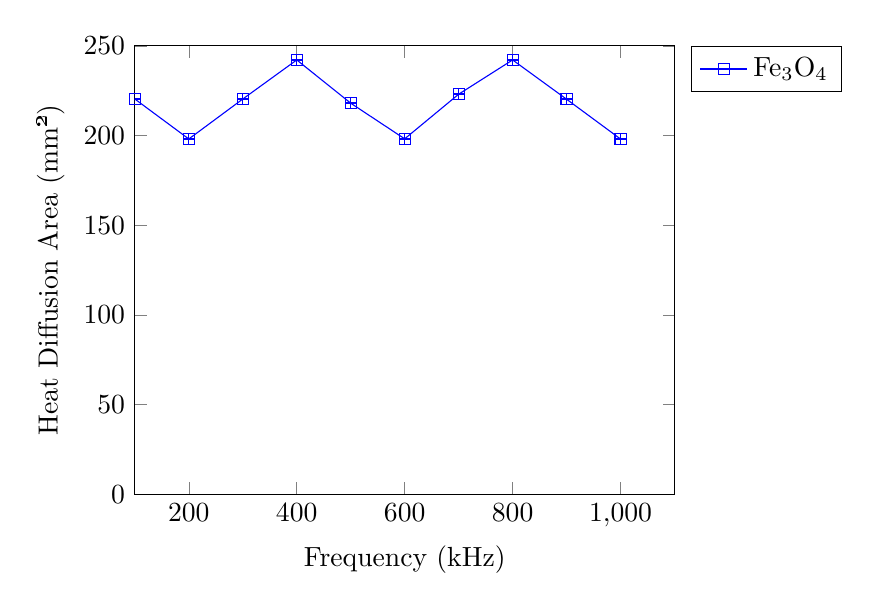
\begin{tikzpicture}
\begin{axis}[
    xlabel={Frequency (kHz)},
    ylabel={Heat Diffusion Area (mm²)},
    xmin=100, xmax=1100,
    ymin=0, ymax=250,
    legend pos=outer north east,
    grid style=dashed,
]

\addplot+[blue, mark=square, error bars/.cd, x dir=both, x fixed=0.001, y dir=both, y fixed=0.1] 
coordinates {
    (100,220.32)(200,198.05)(300,220.33)(400,242.12)(500,218.01)(600,198.12)(700,223.01)(800,242.12)(900,220.22)(1000,198.02)
};
\legend{\ce{Fe3O4}} 
\end{axis}
\end{tikzpicture}
    \caption{Heat Generated (SAR $\pm 0.1$ ) vs frequency (kHz $\pm 0.001$) for \ce{Fe3O4}}
    \label{fig:feheatgeneration}
\end{figure}

\FloatBarrier
\begin{figure}[h!]
    \centering
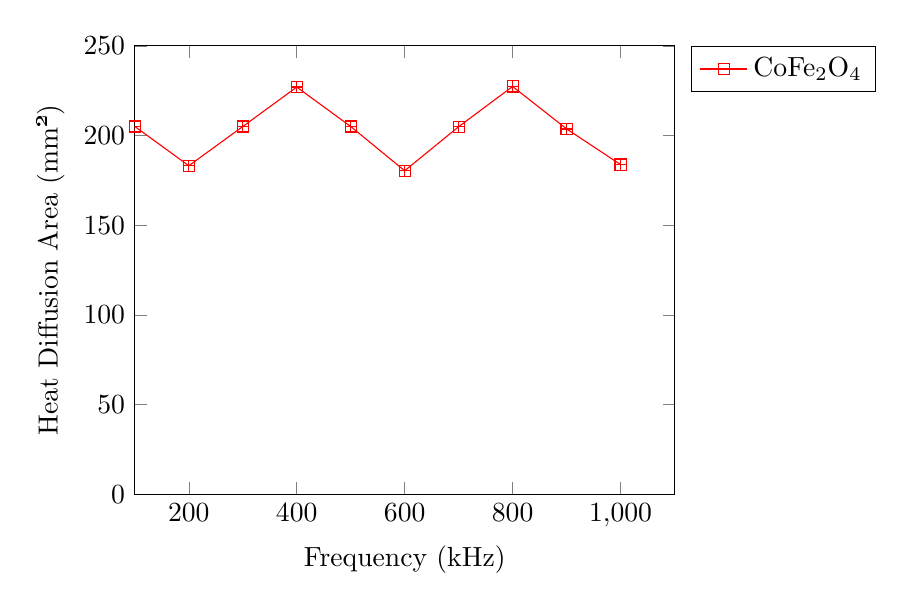
\begin{tikzpicture}
\begin{axis}[
    xlabel={Frequency (kHz)},
    ylabel={Heat Diffusion Area (mm²)},
    xmin=100, xmax=1100,
    ymin=0, ymax=250,
    legend pos=outer north east,
    grid style=dashed,
]

\addplot+[red, mark=square, error bars/.cd, x dir=both, x fixed=0.001, y dir=both, y fixed=0.1] 
coordinates {
    (100,205)
    (200,183.12)
    (300,205)
    (400,227)
    (500,205)
    (600,180.33)
    (700,204.89)
    (800,227.32)
    (900,203.66)
    (1000,183.77)
};
\legend{\ce{CoFe2O4}} 
\end{axis}
\end{tikzpicture}
    \caption{Heat Generated (SAR $\pm 0.1$ ) vs frequency (kHz $\pm 0.001$) for \ce{CoFe2O4}}
    \label{fig:coheatgeneration}
\end{figure}

\FloatBarrier
\begin{figure}[h!]
    \centering
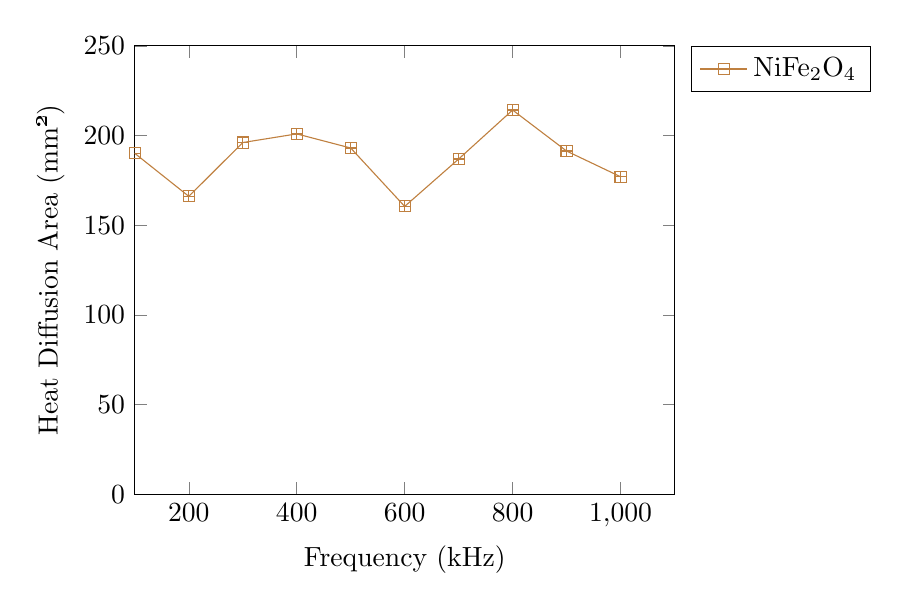
\begin{tikzpicture}
\begin{axis}[
    xlabel={Frequency (kHz)},
    ylabel={Heat Diffusion Area (mm²)},
    xmin=100, xmax=1100,
    ymin=0, ymax=250,
    legend pos=outer north east,
    grid style=dashed,
]

\addplot+[brown, mark=square, error bars/.cd, x dir=both, x fixed=0.001, y dir=both, y fixed=0.1] 
coordinates {
      (100,190)(200,166.05)(300,196.06)(400,200.88)(500,193)(600,160.45)(700,186.87)(800,214.18)(900,191.32)(1000,176.99)
};
\legend{\ce{NiFe2O4}} 
\end{axis}
\end{tikzpicture}
    \caption{Heat Generated (SAR $\pm 0.1$ ) vs frequency (kHz $\pm 0.001$) for \ce{NiFe2O4}}
    \label{fig:niheatgeneration}
\end{figure}

\FloatBarrier
\begin{figure}[h!]
    \centering
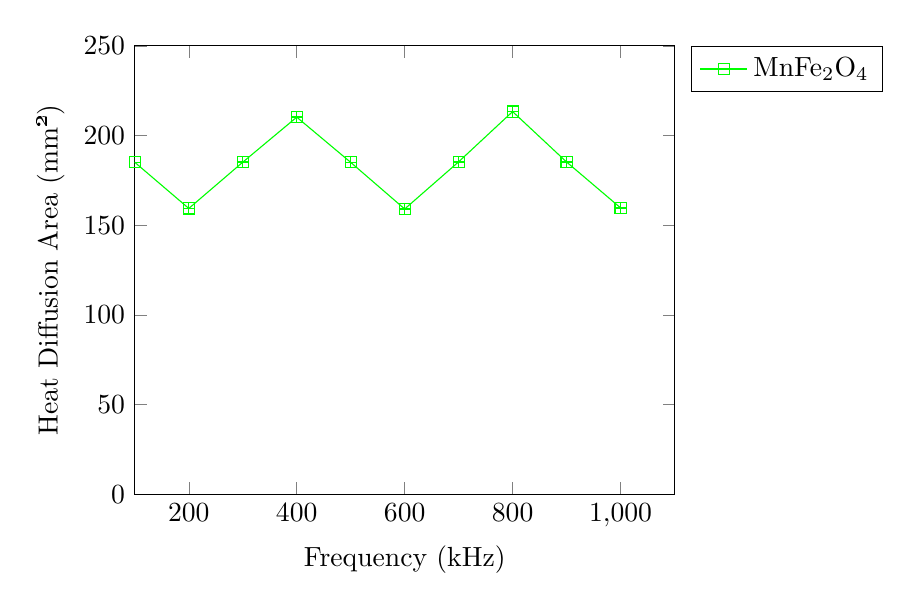
\begin{tikzpicture}
\begin{axis}[
    xlabel={Frequency (kHz)},
    ylabel={Heat Diffusion Area (mm²)},
    xmin=100, xmax=1100,
    ymin=0, ymax=250,
    legend pos=outer north east,
    grid style=dashed,
]

\addplot+[green, mark=square, error bars/.cd, x dir=both, x fixed=0.001, y dir=both, y fixed=0.1] 
coordinates {
   (100,185.0)(200,159.31)(300,185.12)(400,210.22)(500,185)(600,159)(700,185.32)(800,213.32)(900,185.21)(1000,159.64)
};
\legend{\ce{MnFe2O4}} 
\end{axis}
\end{tikzpicture}
    \caption{Heat Generated (SAR $\pm 0.1$ ) vs frequency (kHz $\pm 0.001$) for \ce{MnFe2O4}}
    \label{fig:mnheatgeneration}
\end{figure}

\FloatBarrier
\begin{figure}[h!]
    \centering
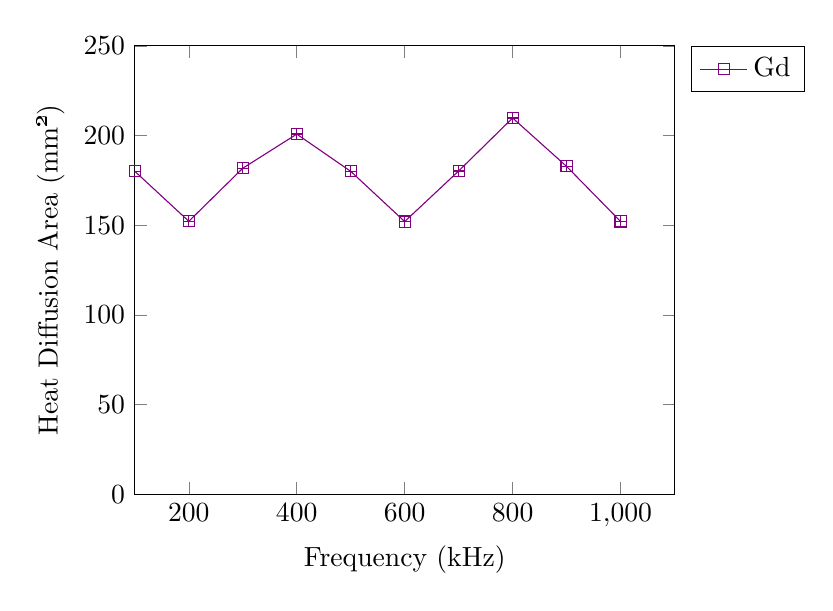
\begin{tikzpicture}
\begin{axis}[
    xlabel={Frequency (kHz)},
    ylabel={Heat Diffusion Area (mm²)},
    xmin=100, xmax=1100,
    ymin=0, ymax=250,
    legend pos=outer north east,
    grid style=dashed,
]

\addplot+[violet, mark=square, error bars/.cd, x dir=both, x fixed=0.001, y dir=both, y fixed=0.1] 
coordinates {
    (100,180)(200,152.15)(300,181.73)(400,200.76)(500,180)(600,152)(700,180.19)(800,209.76)(900,182.76)(1000,152.06)
};
\legend{\ce{Gd}} 
\end{axis}
\end{tikzpicture}
    \caption{Heat Generated (SAR $\pm 0.1$ ) vs frequency (kHz $\pm 0.001$) for Gd}
    \label{fig:gdheatgeneration}
\end{figure}

\newpage
\FloatBarrier
\printbibliography
\end{document}
